% Chapter Template

\chapter{Network Geometry} % Main
% chapter title

\label{Chapter-Network} % Change X to a consecutive number; for
% referencing this chapter elsewhere, use \ref{ChapterX}

\lhead{Chapter 4. \emph{Network Analysis}} % Change X to a consecutive number; this is for the header on each page - perhaps a shortened title

\section{Skeletonization}

The skeleton of an object is a representation of the object, which contain both,
shape features and topological structures of the original object. It is widely
used in computer graphics, character recognition, and analysis of biomedical
images.\citep{bai_skeleton_2007,golland_fixed_2000,ge_generation_1996}. A fundamental property required by thinning algorithms is that the topology of the object is preserved. Informally, two objects have the same topology if one can be deformed into another applying only continuous deformations (no cutting, no gluing). For example, a donut and a cup of coffee share the same topology. Holes modify the topology of the object. Any set without holes is homotopic to a single point in that space.

The skeletonization has to conserve topology, but also shape features. If we are only concerned about topology, we have an ultimate skeleton, it reduces set of points to the simplest set with the same topology. Again, any object without holes will be reduced to single point, objects with one hole to circles/donuts. The shape features to conserve depend on the purpose of the skeleton, a typical case to conserve shapes is to keep end-points that are only connected to one point, i.e only one neighbor. The removal of these end-points would still conserve topology but the shape will be lost.

The skeletonization is very sensitive to noise and boundary deformations, which generates redundant skeleton branches. (Fig.\ref{fig:skeleton-fixedtopo-network}(b)).

To overcome this instability, the methods used are based on skeleton pruning, i.e. eliminating the spurious branches.

\begin{figure}[ht]
\centering
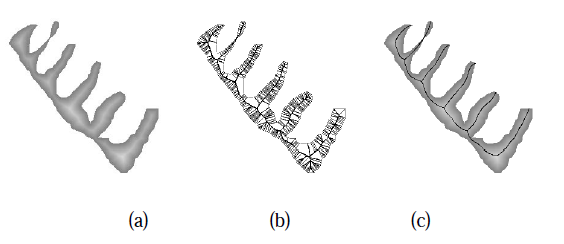
\includegraphics[width=0.8\textwidth]{Figures/chapter-network/skeleton-fixedtopo_letters.png}%
\caption[Skeletonization]{Skeletonization process. (a) Distance
map. (b) Traditional skeleton with no pruning. (c) Skeleton generated using
fixed topology methods. From Ref.\citep{bai_skeleton_2007,golland_fixed_2000}}
\label{fig:skeleton-fixedtopo-network}
\end{figure}

The pruning of spurious branches is usually made by discarding branches that are shorter than a fixed amount of pixels. This parameter should be chosen by the user to keep important information about the structure, but removing noisy and spurious branches. Like any other threshold-based method, the perfect value for the threshold is unknowable, and in most cases, unachievable, no matter how sophisticated is the algorithm in use. Having said that, a good enough threshold is easy to achieve checking the results of the skeletonization using the human brain. Algorithms using human feedback are usually called guided or supervised.

Recently in the literature, a method was proposed with an alternative approach for the pruning of spurious branches \cite{couprie_3d_2015, bertrand_parallel_2017} using a persistence parameter to keep branches that are important. I have contributed this skeletonization method to the open source library DGTal, see \autoref{Appendix-Contributions}.

